\thispagestyle{quantoannone}
\pagestyle{quantoan}
\everymath{\color{quantoan}}
\graphicspath{{../quantoan/pic/}}
%\blfootnote{\color{quantoan}\color{quantoan}$^*$Nguồn Math. Intellegencer, Số $41$.}
\begingroup
\AddToShipoutPicture*{\put(0,616){\includegraphics[width=19.3cm]{../bannerquantoan}}}
\AddToShipoutPicture*{\put(72,523){\includegraphics[scale=1]{../tieude1.pdf}}}
\centering
\endgroup
\vspace*{185pt}

\begin{multicols}{2}
	``\textit{Xin đừng xáo trộn những vòng tròn của tôi}"
	\vskip 0.1cm
	\hfill Μὴ μου τοὺς κύκλους τάραττε (tiếng Hy lạp)
	\vskip 0.1cm
	\hfill Noli turbare circulos meos (Tiếng La tinh)
	\vskip 0.1cm
	Khi chúng ta còn nhỏ, chắc hẳn ai cũng đều nghe tới chuyện, có một ông già thời cổ đại nào đó, ông ta ngồi trên bờ biển, đang vẽ một cái hình gì đó trên cát thì một người lính cưỡi ngựa đi qua và vô tình đâm chiếc giáo làm ông già ngã xuống, ông ấy chỉ kịp thốt lên ``ôi, làm ơn đừng làm hỏng những hình vẽ của tôi".
	\begin{figure}[H]
		\vspace*{-5pt}
		\centering
		\captionsetup{labelformat= empty, justification=centering}
		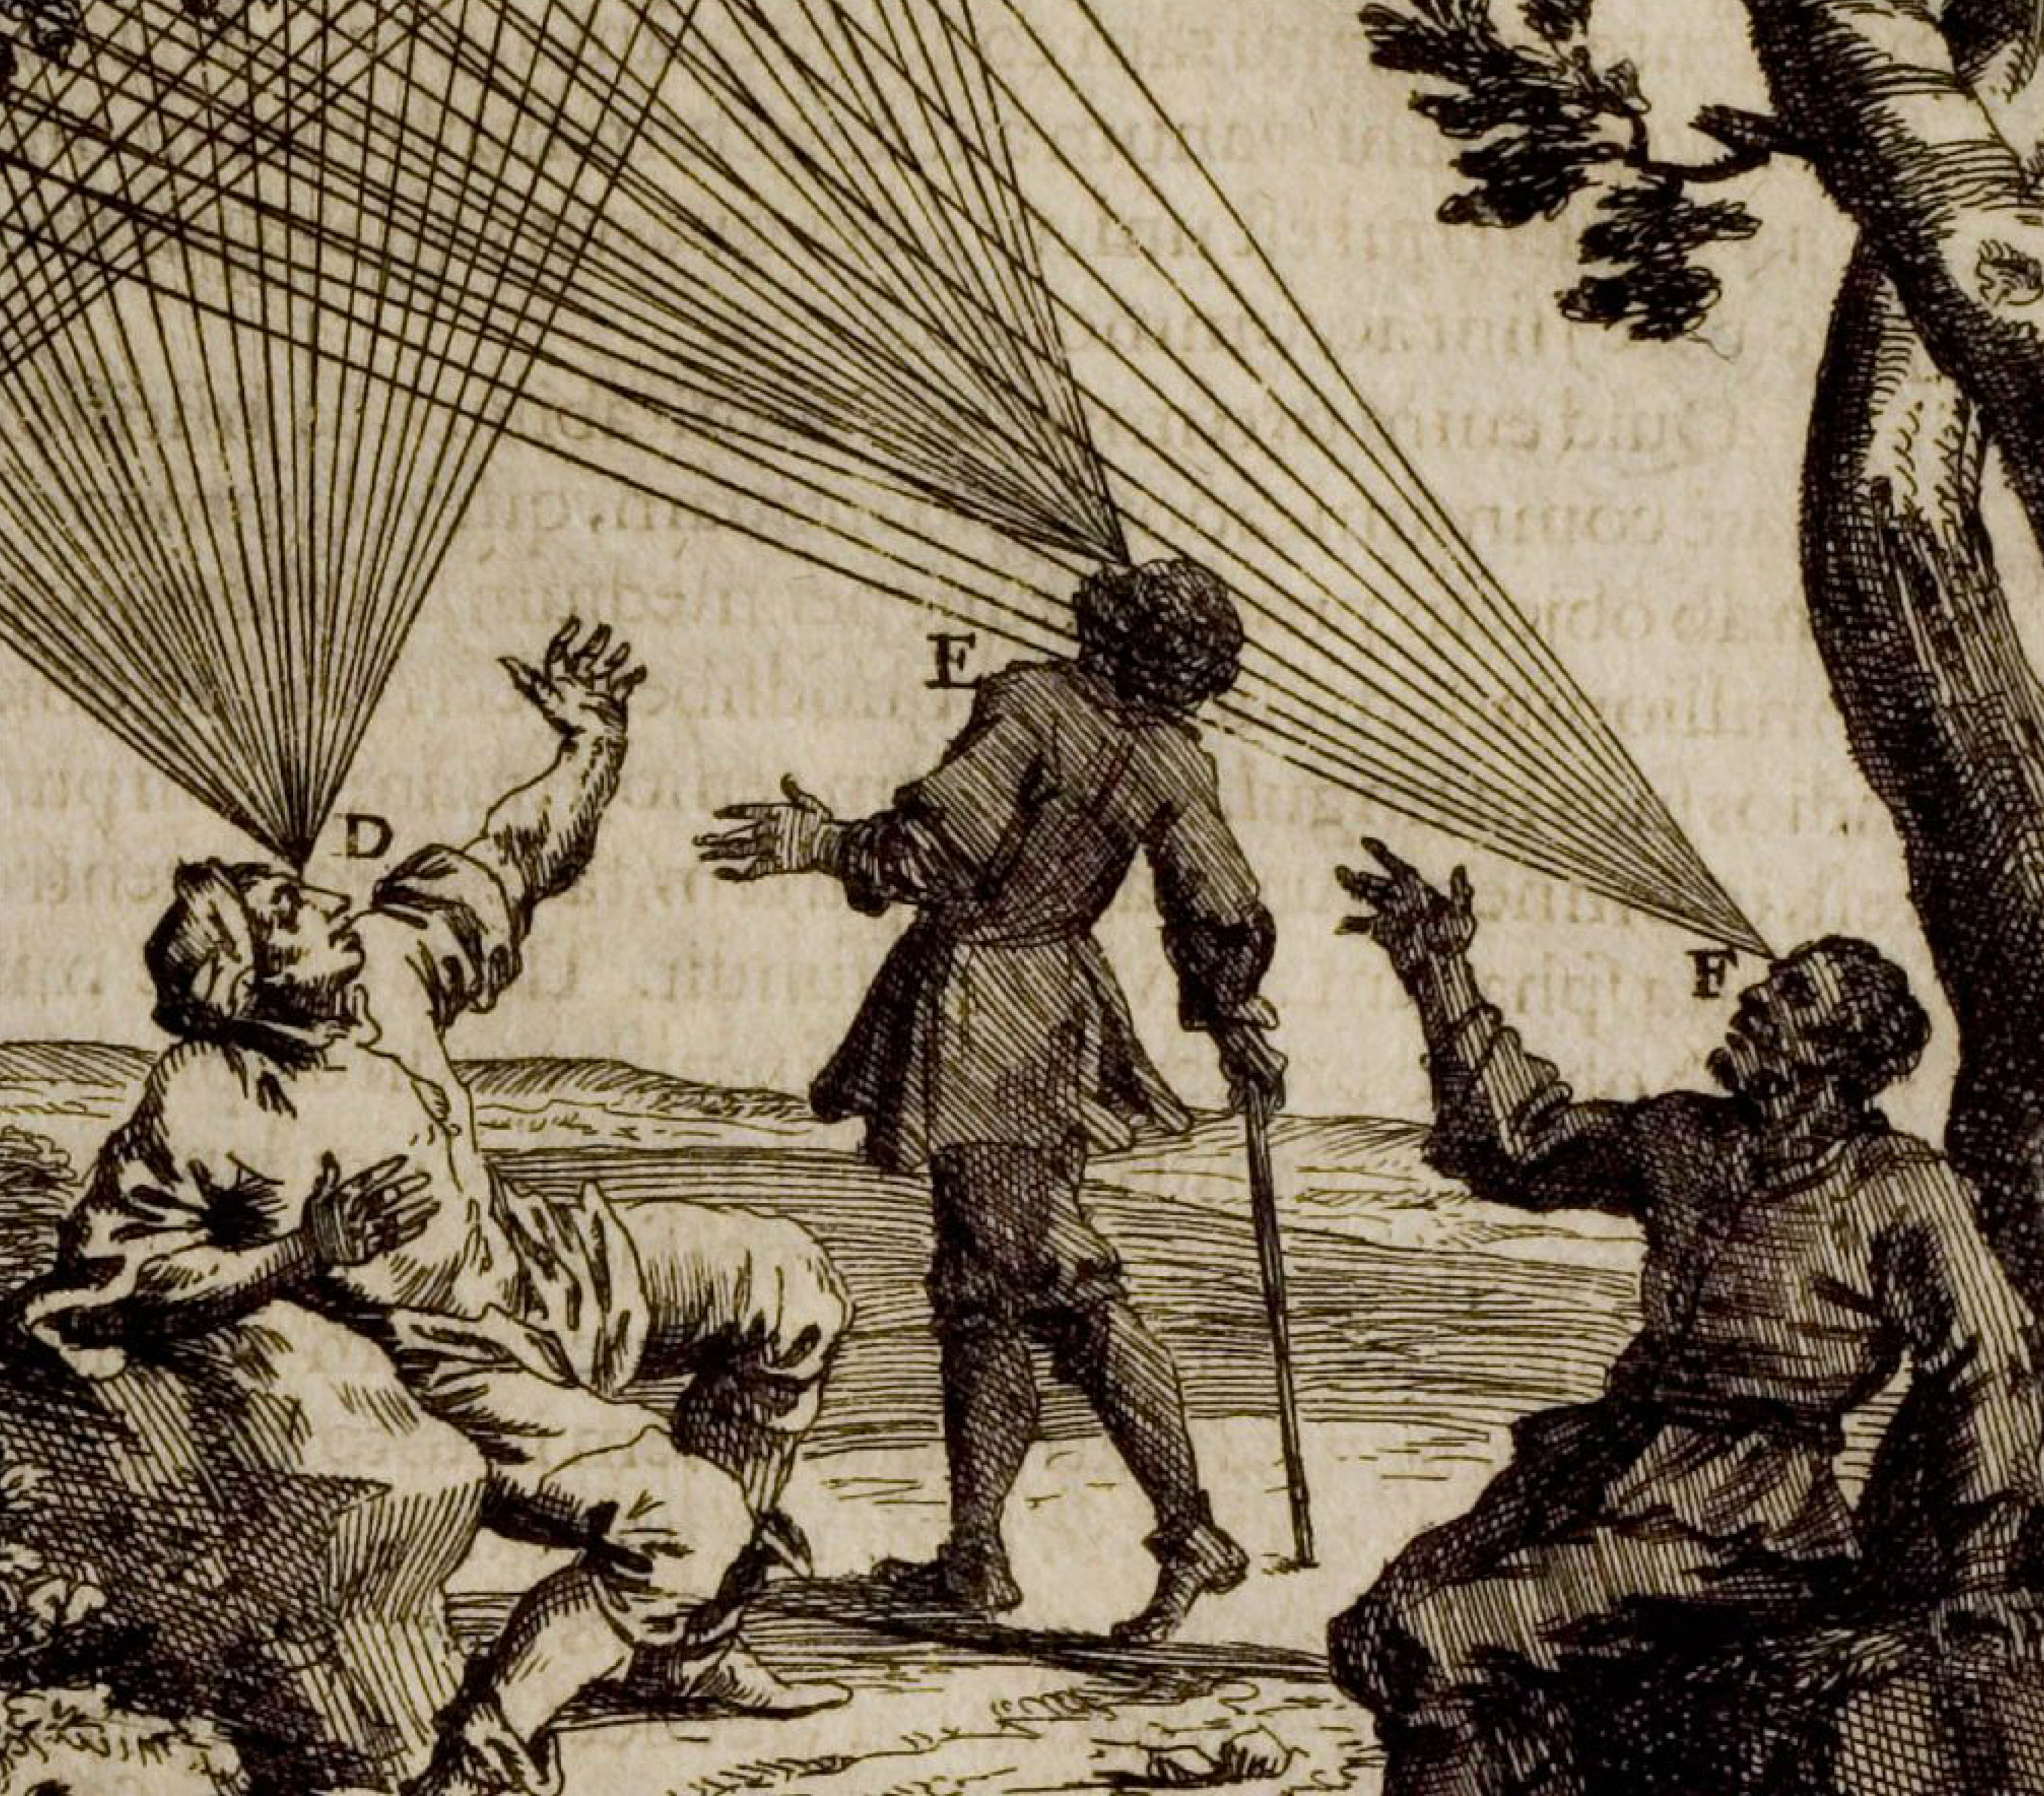
\includegraphics[width= 1\linewidth]{1}
%		\caption{\small\textit{\color{}}}
		\vspace*{-15pt}
	\end{figure}
	Câu chuyện này làm chúng ta mê say tới mức, lúc còn thơ ấu, cứ mỗi lần bạn và tôi đi nghỉ hè ở biển, chúng ta đều cố thử ngồi trên cát trắng và vẽ những hình tam giác, hình tròn và đợi những ngọn sóng ập tới xoá đi nhanh chóng những ký hoạ tạo ra trong những hình dung đẹp đẽ mơ hồ của chũng ta về một môn học gọi là Toán.
	\vskip 0.1cm
	Rồi tới khi học Vật lý, chúng ta lại được biết tới một ông già nào đó khác ở một xứ nọ, ông đang ngồi ngâm mình trong bồn tắm thì bỗng vùng dậy chạy ra đường và kêu lên: Eureka! Tất cả các bạn bè của chúng ta đều yêu mến câu chuyện đó, và đều hay thốt lên một cách hồn nhiên "Eureka!" khi muốn nói đến một khám phá bất chợt, giống như khi giải ra được một bài toán khó vào chiều tối thứ Sáu.
	\vskip 0.1cm
	Các câu chuyện trên đều về một người, đó là Archimedes xứ Syracuse ($287-212$). Về cái chết của ông, Wikipedia có viết ngắn gọn như sau: ``Archimedes chết trong đợt vây hãm thành Syracuse, ở đó ông bị một người lính La Mã giết mặc dù có mệnh lệnh phải bảo toàn tính mạng cho Archimedes." Vào lúc đó, Archimedes,  nổi tiếng với trí tuệ kiến thức uyên thâm về hình học và cơ học, đã làm cho tướng quân La Mã là Marcus Claudius Marcellus phải nể phục. Marcellus biết rằng mình đã phải nhọc nhằn như thế nào trong việc chinh phục thành Syracuse cũng do các cỗ máy cơ học tinh xảo mà Archimedes chế tạo đã giúp dân thành chống cự được lính La Mã thiện chiến. Người La Mã nổi tiếng với tính tàn ác lạnh lùng, nhưng cũng là những người đề cao danh dự chiến trường. Vì quá hâm mộ tài năng đột xuất của Archimedes, tướng quân Marcellus ra lệnh phải giữ mạng sống cho nhà toán học -- đối với Marcellus, cứu được Archimedes cũng đáng được  vinh quang như hạ được thành luỹ của Syracuse bằng gươm kiếm.
	\vskip 0.1cm
	Tuy nhiên, một người lính được cử đến để yêu cầu Archimedes nộp mình làm tù binh cho quân La Mã đã làm hỏng kế hoạch tỷ mỷ mà Marcellus nghĩ ra. Anh ta thô lỗ đạp cửa đột nhập vào nhà của Archimedes, đúng lúc  nhà toán học đang trầm ngâm mải mê vẽ những hình vẽ phức tạp. Người lính tuốt kiếm ra và hỏi Archimedes tên ông là gì. Archimedes vì đang mải miết với công việc, không nhận thấy ai đang chỉ kiếm về mình, đã nói với người lính ``Xin làm ơn đừng có làm xáo trộn những hình vẽ của tôi, anh bạn ơi!". Ông còn hét lên ``Ai đưa giúp cho tôi một trong những cái máy của tôi nào!" Người lính La Mã, vì quá sợ hãi, theo bản năng tự vệ bèn đâm thẳng kiếm vào ông già yếu ớt, và cũng trong giây phút ấy, đã hạ gục nhà toán học vĩ đại.
	\vskip 0.1cm
	Nhưng vì sao lại có câu chuyện về Archimedes bị đâm chết khi ngồi trên bãi cát nhỉ? Phần lớn các tài liệu đều đồng ý, ông đang ngồi tại nhà riêng và đang vẽ những hình hình học thì bị người lính đột nhập tới đâm ông bằng kiếm. Lúc đó Archimedes đang sử dụng một công cụ là bảng vẽ abax, một dụng cụ để vẽ bằng bụi cát. Vì vậy mới có dị bản trên về bãi cát như tôi và các bạn đã từng nghe khi còn nhỏ.
	\begin{figure}[H]
		\vspace*{-5pt}
		\centering
		\captionsetup{labelformat= empty, justification=centering}
		\includegraphics[width= 1\linewidth]{2}
%		\caption{\small\textit{\color{}}}
		\vspace*{-15pt}
	\end{figure}
	Ân hận với hành động bất cẩn của quân lính, Marcellus đã xin lỗi họ hàng của Archimedes và cho đặt trên mộ của ông một biểu tượng mô tả một hình cầu đặt trong một hình trụ, và mãi $137$ năm sau, một nhà chính trị gia La Mã là Cicero mới tìm thấy ngôi mộ này của nhà toán học. Người La Mã cổ đại nói chung không quan tâm tới toán học, và hành động dọn dẹp ngôi mộ cho phong quang của Cicero có lẽ là đóng góp đáng ghi nhớ nhất của bất kỳ người La Mã nào đối với lịch sử phát triển của toán học.
	\begin{figure}[H]
		\vspace*{-5pt}
		\centering
		\captionsetup{labelformat= empty, justification=centering}
		\includegraphics[width= 0.8\linewidth]{3}
		\caption{\small\textit{\color{quantoan}Hình $2$. Biểu tượng về hình cầu và hình trụ như thế này đã được khắc trên mộ của Archimedes.}}
		\vspace*{-10pt}
	\end{figure}
	Sự thiên tài và đầu óc luôn muốn tò mò khám phá tri thức của Archimedes tiếp tục truyền cảm hứng tới nhiều nhà tư tưởng khác rất lâu sau khi ông qua đời, từ Galileo cho tới Issac Newton. Chúng ta có thể nhắc tới Sophie Germain, một nữ toán học người Pháp sinh năm $1776$. Vào năm $13$ tuổi, cô đã được đọc câu chuyện về cái chết của Archimedes. Sophie cho rằng bất kỳ môn học nào mà có thể thu hút một người tập trung say mê như vậy, đều đáng để nghiên cứu, và cô quyết định tự học toán -- đặc biệt là môn lý thuyết số. Cha mẹ cô đã lo lắng rất nhiều về sở thích toán học của con gái mình khi cô còn là một cô bé, và vào thời cô sống, việc phụ nữ trở thành một nhà toán học là điều không bình thường, vì vậy họ đã tịch thu tất cả các cây nến của cô và dỡ bỏ mọi thiết bị sưởi ấm trong phòng cô. Cô đáp lại bằng cách bí mật thắp nến rồi ngồi vào bàn, quấn chăn kín người. Cha mẹ cô cuối cùng đã mủi lòng một cách thật thông thái và quyết định tài trợ cho việc học hành của cô. Sophie, sau khi tìm thấy một sinh viên sắp rời Paris tên là Antoine--August Le Blanc, đã bí mật thế chỗ anh ta, sử dụng tên của anh ta để gửi và nhận tài liệu từ Ecole Polytechnic khi đó mới mở,  vì trường chỉ nhận sinh viên nam tới học. Joseph--Louis Lagrange, lúc đó là người hướng dẫn của Sophie, đã rất ngạc nhiên khi  sinh viên này có thể tiến bộ rất nhiều -- từ một học sinh tệ hại trở thành người có bài tập giải hàng tuần (tất nhiên là được gửi qua đường bưu điện) là tốt nhất trong lớp. Lagrange yêu cầu được gặp ``anh" sinh viên Le Blanc và ngạc nhiên khi biết rằng ``Anh" ta hoá ra là một quý ``Cô"! Sophie đã trở thành một trong những nhà lý thuyết số xuất chúng nhất trong thời đại của cô.
	\begin{figure}[H]
		\vspace*{5pt}
		\centering
		\captionsetup{labelformat= empty, justification=centering}
		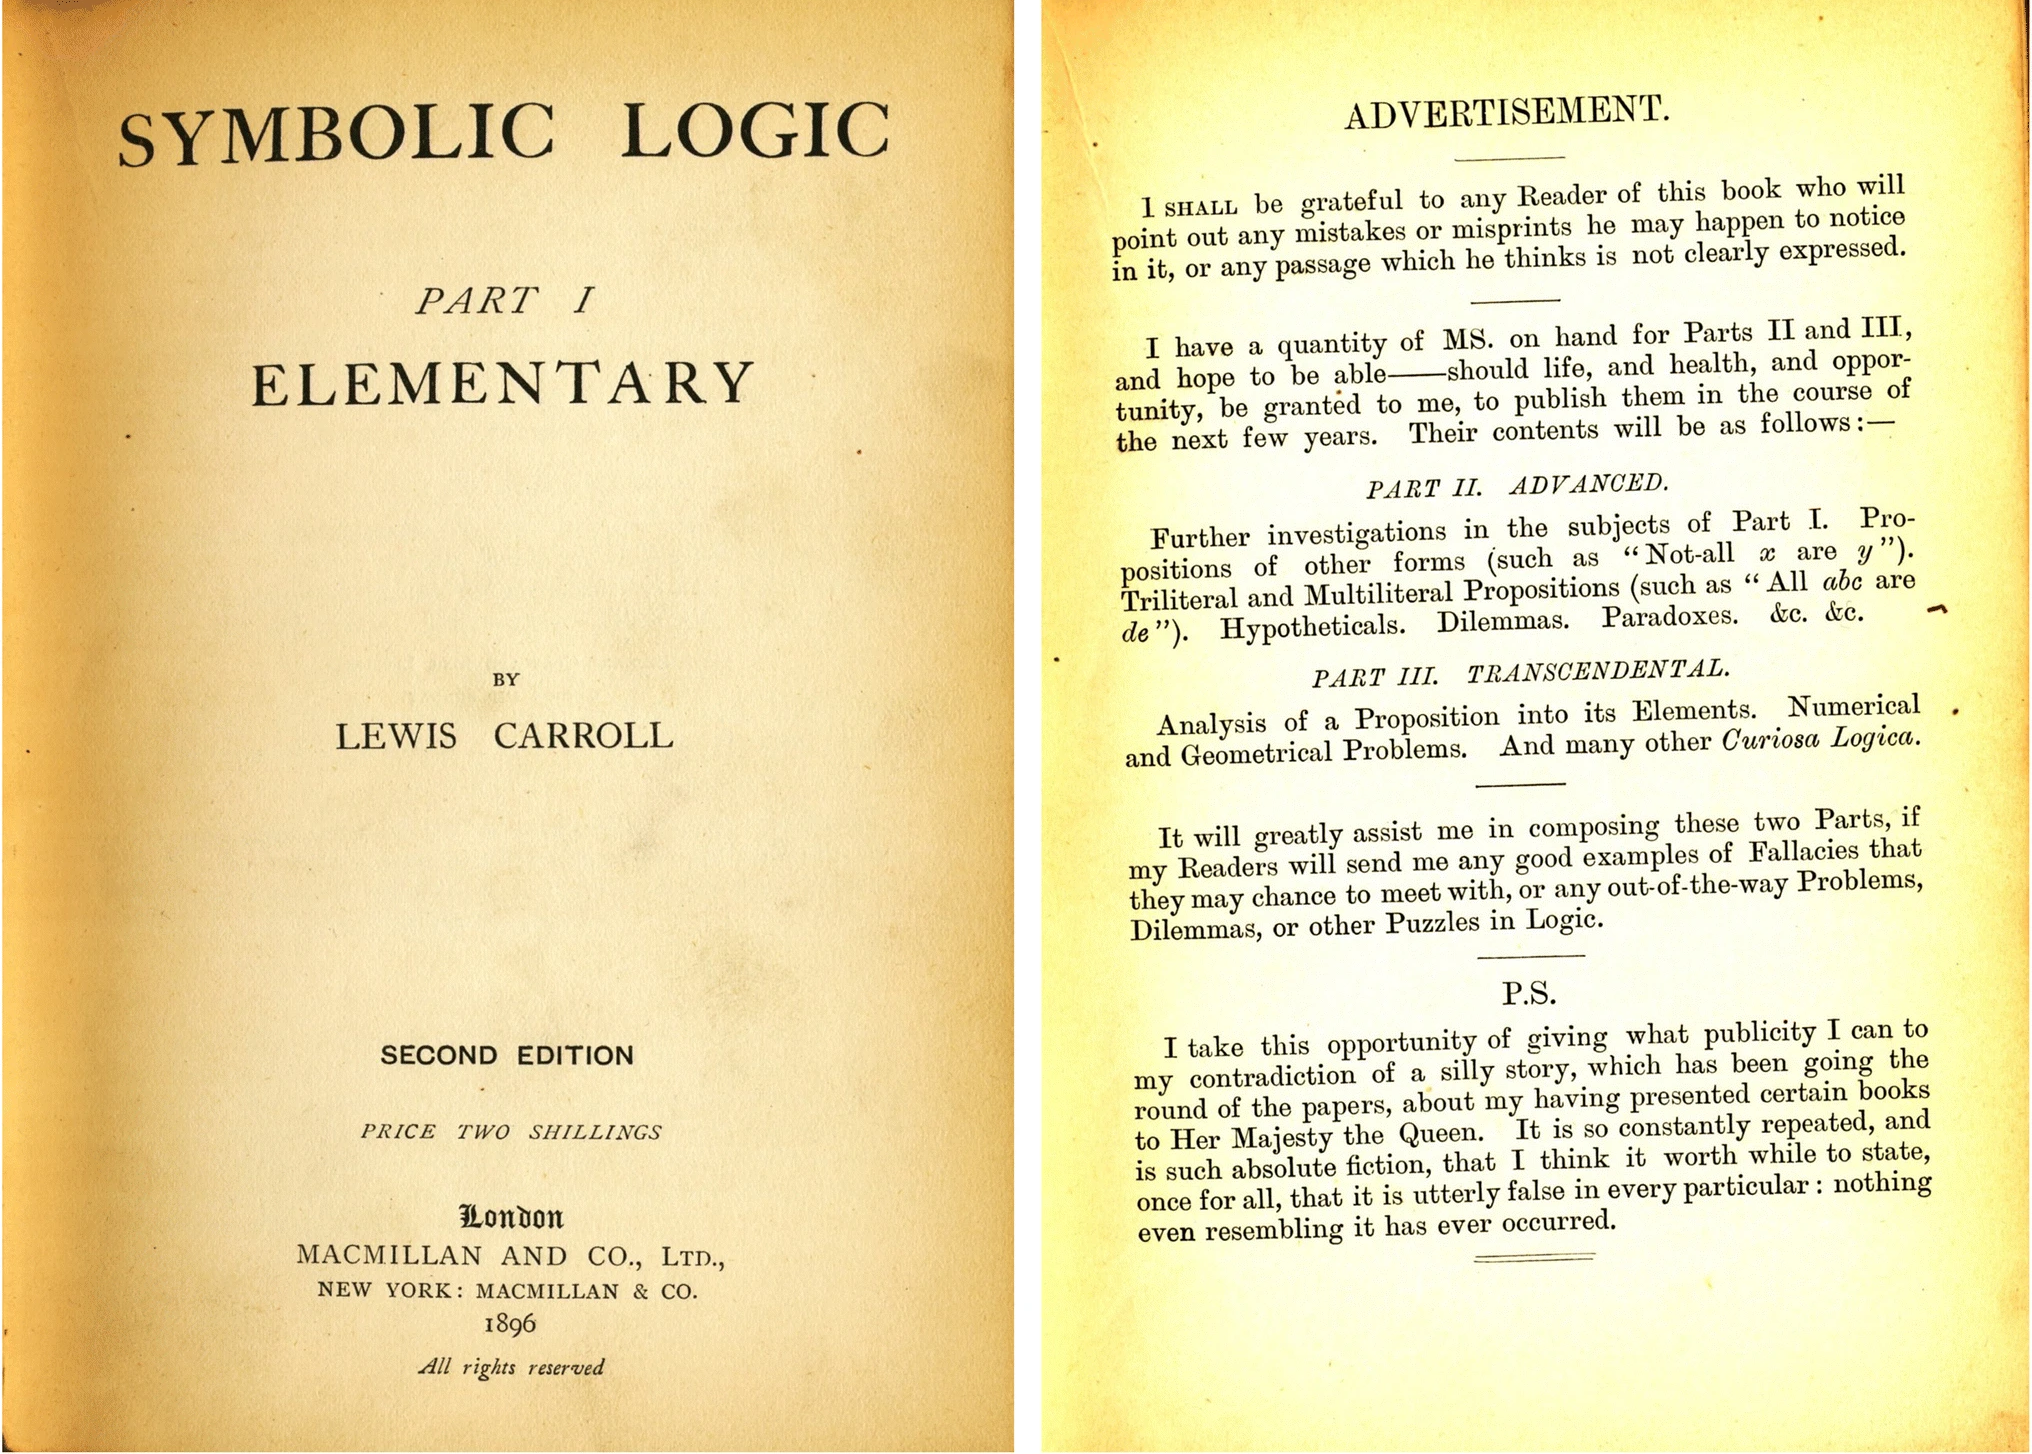
\includegraphics[width= 1\linewidth]{4}
		\caption{\small\textit{\color{quantoan}Hình $3$. Sophie Germain ($1776-1831$) -- Nhà toán học, vật lý học và Triết học gia người Pháp.}}
		\vspace*{-10pt}
	\end{figure}
	Chắc các bạn đọc đến đây đã yêu thích hơn chiếc bàn học ngăn nắp của mình được rọi chiếu bởi ánh sáng thoáng đãng rồi chứ?
	\vskip 0.1cm
	Tham khảo dựa trên các nguồn internet:
	\vskip 0.1cm
	[$1$]	\url{https://math.nyu.edu/~crorres/Archimedes/contents.html}
	\vskip 0.1cm
	[$2$]	\url{https://en.wikipedia.org/w/index.php?title=Archimedes&oldid=1146936468}
	
	
\end{multicols}